\documentclass{article}
\usepackage{tikz}
\usetikzlibrary{arrows.meta}

\begin{document}

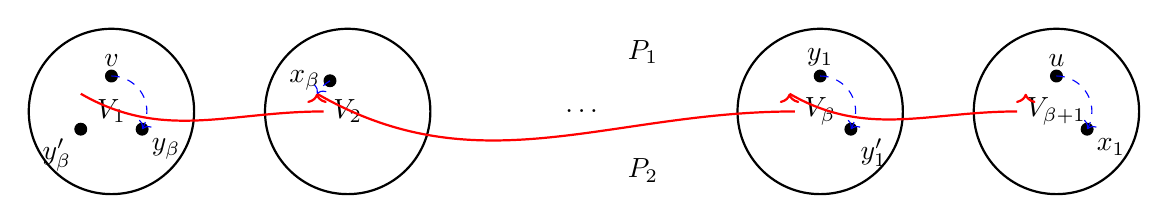
\begin{tikzpicture}[scale=1.5]
    % Define nodes
    \node (V1) at (-2,0) {$V_1$};
    \node (V2) at (0,0) {$V_2$};
    \node (Vb) at (4,0) {$V_\beta$};
    \node (Vbp1) at (6,0) {$V_{\beta+1}$};

    % Draw circles
    \draw[thick] (V1) circle (0.7);
    \draw[thick] (V2) circle (0.7);
    \draw[thick] (Vb) circle (0.7);
    \draw[thick] (Vbp1) circle (0.7);

    % Nodes inside circles
    \filldraw[black] (V1) ++(90:0.3) circle (0.05) node[above] {$v$};
    \filldraw[black] (V1) ++(-30:0.3) circle (0.05) node[below right] {$y_\beta$};
    \filldraw[black] (V1) ++(-150:0.3) circle (0.05) node[below left] {$y'_\beta$};
    \filldraw[black] (V2) ++(120:0.3) circle (0.05) node[left] {$x_\beta$};
    \filldraw[black] (Vb) ++(90:0.3) circle (0.05) node[above] {$y_1$};
    \filldraw[black] (Vb) ++(-30:0.3) circle (0.05) node[below right] {$y'_1$};
    \filldraw[black] (Vbp1) ++(90:0.3) circle (0.05) node[above] {$u$};
    \filldraw[black] (Vbp1) ++(-30:0.3) circle (0.05) node[below right] {$x_1$};

    % Arrows between circles
    \draw[->, thick, red] (V1) ++(150:0.3) to[out=-30,in=180] (V2) ++(150:0.3);
    \draw[->, thick, red] (V2) ++(150:0.3) to[out=-30,in=180] (Vb) ++(150:0.3);
    \draw[->, thick, red] (Vb) ++(150:0.3) to[out=-30,in=180] (Vbp1) ++(150:0.3);

    % Dashed arrows within circles
    \draw[dashed, blue, ->] (V1) ++(90:0.3) arc (90:-30:0.3);
    \draw[dashed, blue, ->] (V2) ++(120:0.3) arc (120:150:0.3);
    \draw[dashed, blue, ->] (Vb) ++(90:0.3) arc (90:-30:0.3);
    \draw[dashed, blue, ->] (Vbp1) ++(90:0.3) arc (90:-30:0.3);

    % Labels for paths
    \node at (2,0) {\dots};
    \node at (2.5,0.5) {$P_1$};
    \node at (2.5,-0.5) {$P_2$};
\end{tikzpicture}

\end{document}